The \textit{triply-randomized negative binomial beta} (TNBBeta) distribution \citep{lederman2026triplyrandomizednegativebinomialbeta}
is defined on the unit interval with the following density:
\begin{align*}
    \text{TNBBeta}(y; p, q, \varepsilon) &= \text{Beta}(\varepsilon, \varepsilon)\left[\frac{1 - q}{y(1 - y)}\gamma(y, p)\right]^{\varepsilon}\left[1 - 4q\gamma(y, p)\right]^{-\left(\varepsilon + \frac{1}{2}\right)} \\
    \gamma(y, p) &= \frac{1}{4}\operatorname{sech}^2\left(\frac{\operatorname{logit}(y) - \operatorname{logit}(p)}{2}\right)
\end{align*}
where $p \in (0, 1)$ governs the median, $q \in [0, 1)$ governs the concentration about $p$, and $\varepsilon > 0$
controls both concentration about $p$ and tail behavior of the distribution. By scaling a TNBBeta random variable to
the interval $[-1, 1]$ and applying \Cref{alg:tnbbeta-sample}, we are able to produce another rotationally-symmetric
distribution on the unit hypersphere, which we refer to as the SphericalTNBBeta distribution.

\Cref{fig:pq-ablation} and \Cref{fig:p-epsilon-ablation} illustrate some examples of the SphericalTNBBeta distribution over
$\mathbb{S}^2$.
\begin{figure}[H]
    \centering
    \begin{minipage}[t]{0.48\textwidth}
        \centering
        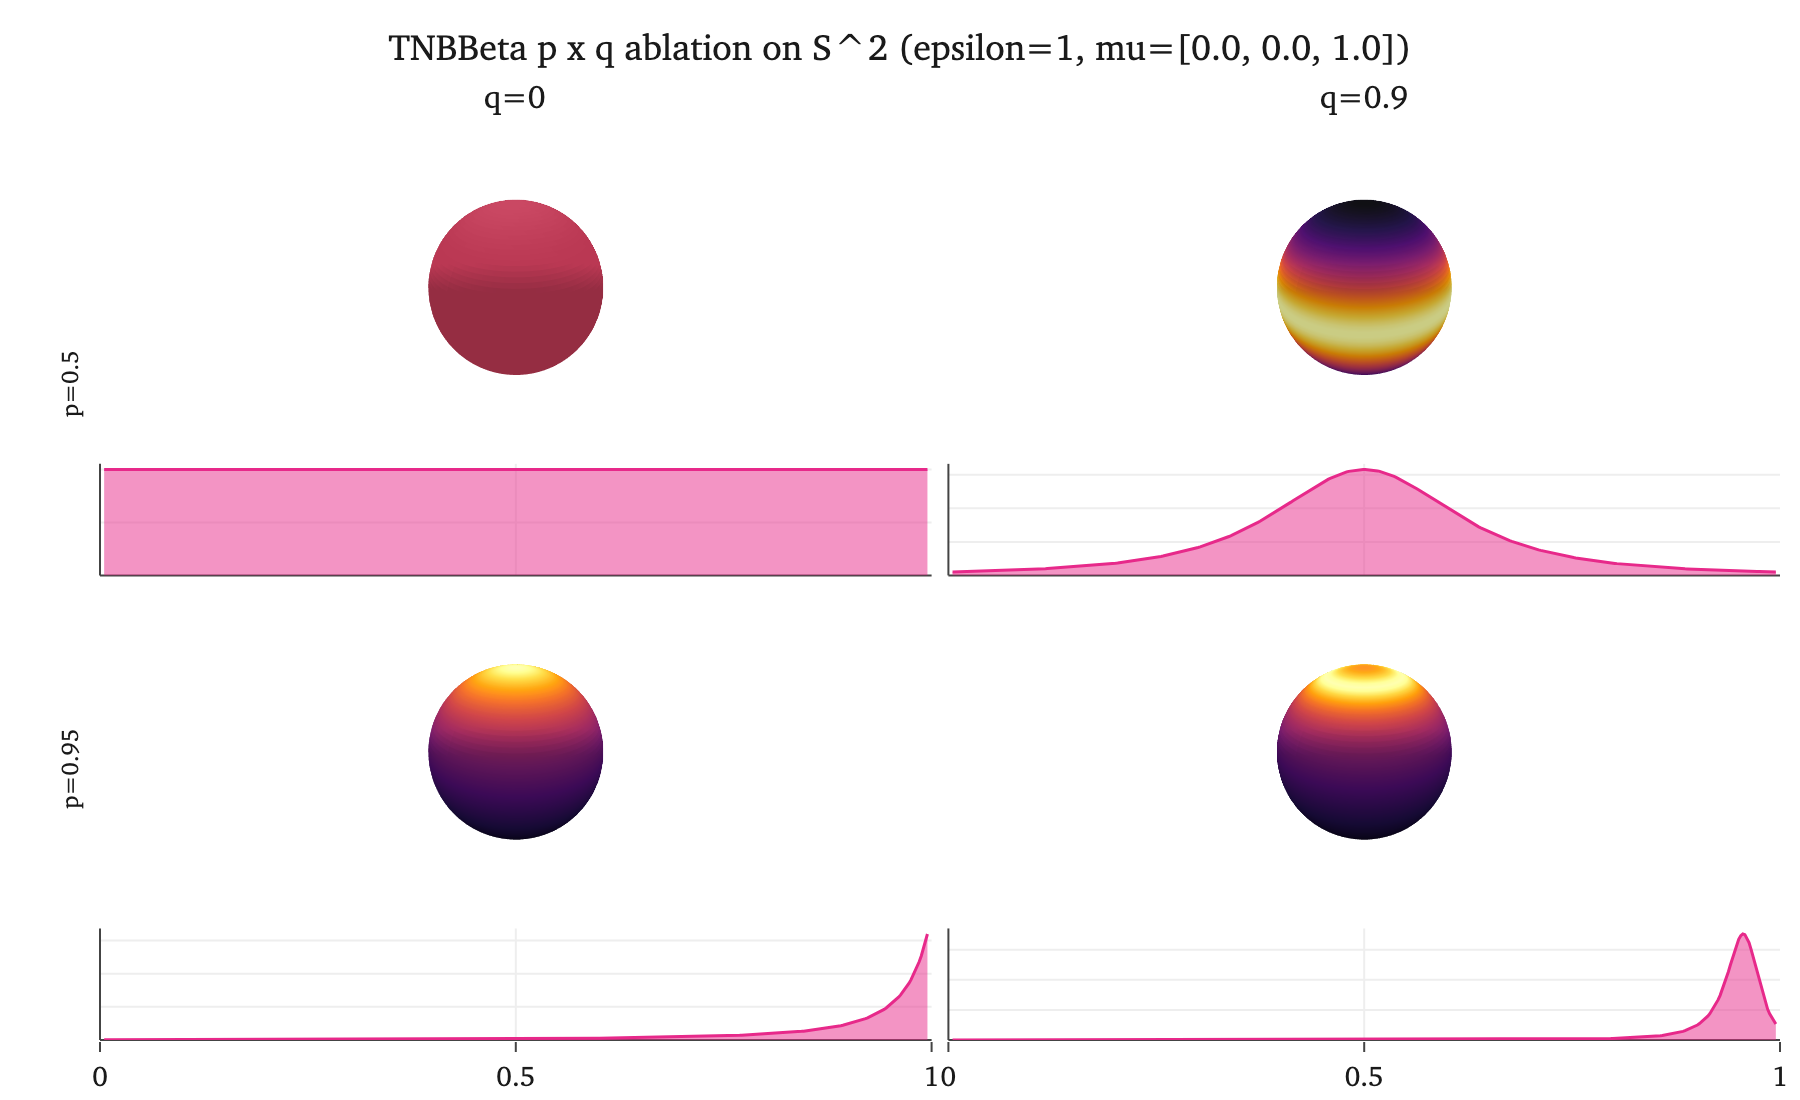
\includegraphics[width=\textwidth]{assets/pq_ablation_2x2.png}
        \captionsetup{width=\linewidth}
        \captionof{figure}{SphericalTNBBeta on $\mathbb{S}^2$ across $p \in \{0.5, 0.95\}$ and $q \in \{0, 0.9\}$
        ($\varepsilon = 1$ fixed): a log-density heatmap above its univariate density below.}
        \label{fig:pq-ablation}
    \end{minipage}
    \hfill
    \begin{minipage}[t]{0.48\textwidth}
        \centering
        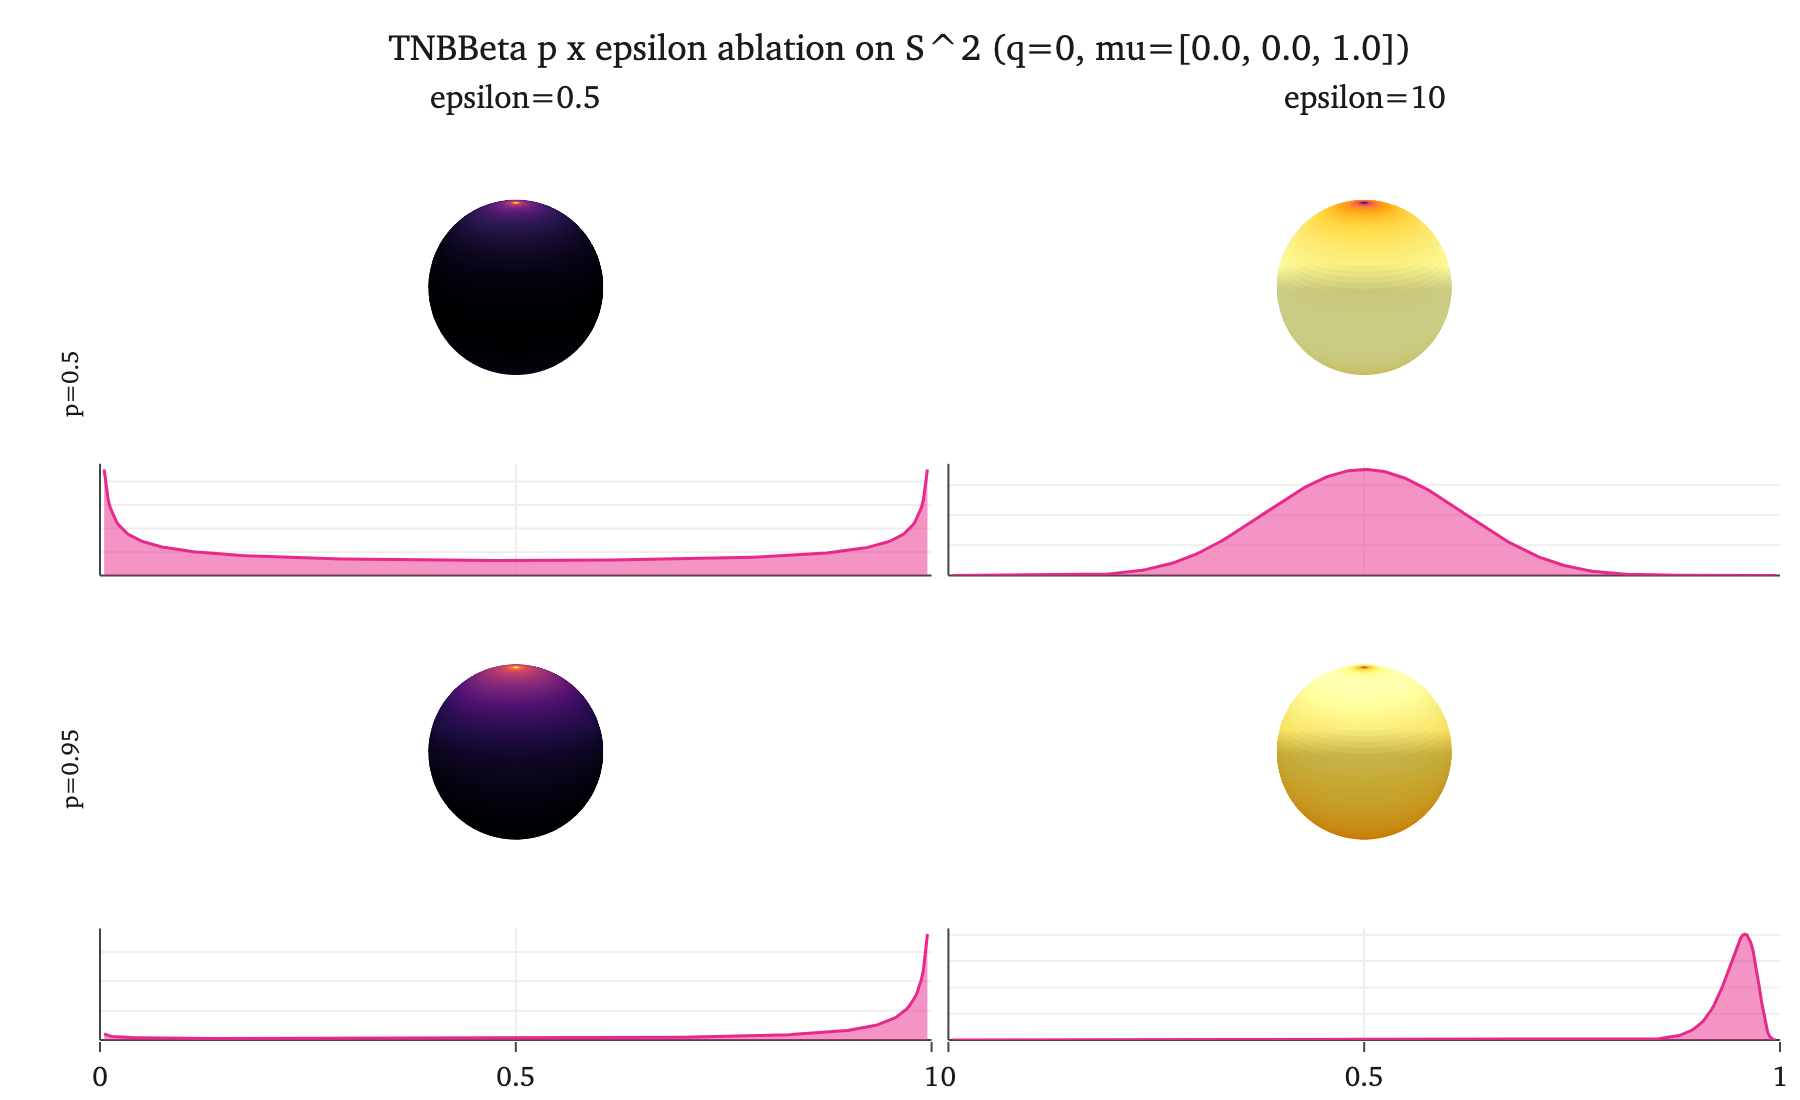
\includegraphics[width=\textwidth]{assets/p_epsilon_ablation_2x2.png}
        \captionsetup{width=\linewidth}
        \captionof{figure}{SphericalTNBBeta on $\mathbb{S}^2$ across $p \in \{0.5, 0.95\}$ and
        $\varepsilon \in \{0.5, 10\}$ ($q = 0$ fixed): $\varepsilon = 0.5$ shows antipodal bimodality,
        $\varepsilon = 10$ shows unimodal concentration.}
        \label{fig:p-epsilon-ablation}
    \end{minipage}
\end{figure}
The bottom-left heatmap of \Cref{fig:pq-ablation} closely resembles the cap-like shape of a vMF or
power-spherical distribution, and this resemblance holds, specifically as $p$ approaches 1:
\begin{theorem}[Limiting behavior of the SphericalTNBBeta distribution]
\label{thm:limiting-tnbbeta}
Suppose $\varepsilon > (d - 1) / 2$. As $p \to 1$, the $\mathrm{SphericalTNBBeta}(\mathbf{x}; \boldsymbol{\mu}, p, q, \varepsilon)$
distribution converges to a dirac mass about $\boldsymbol{\mu}$ and its mass is concentrated within $O(1 - p)$ of $\boldsymbol{\mu}$.
\end{theorem}
As \Cref{fig:pq-ablation} and \Cref{fig:p-epsilon-ablation} show, though, the SphericalTNBBeta distribution is capable of
expressing more shapes, as well as admitting two or more modes. This notion is formalized in \Cref{thm:modality-tnbbeta}.
\begin{theorem}[Modality of the SphericalTNBBeta distribution]
\label{thm:modality-tnbbeta}
For any $p \in (0, 1)$ and $q \in [0, 1)$,
\begin{itemize}
    \item If $\varepsilon > (d - 1) / 2$, $\mathrm{SphericalTNBBeta}(\mathbf{x}; \boldsymbol{\mu}, p, q, \varepsilon)$ is unimodal
    \item If $\varepsilon < (d - 1) / 2$, $\mathrm{SphericalTNBBeta}(\mathbf{x}; \boldsymbol{\mu}, p, q, \varepsilon)$ has at least
    two modes, two of which are located at $\pm \boldsymbol{\mu}$
\end{itemize}
\end{theorem}
Finally, it is important to note that the TNBBeta distribution can be sampled via a deterministic transformation of a single beta-distributed
sample. Hence, given a more expressive density shape, as well as the ability to employ gradient reparametrization, the
SphericalTNBBeta makes for an interesting choice of posterior for a hyperspherical variational autoencoder.